% Component Diagram cho Entity Extraction Pipeline
% Sử dụng trong LaTeX với % Component Diagram cho Entity Extraction Pipeline
% Sử dụng trong LaTeX với % Component Diagram cho Entity Extraction Pipeline
% Sử dụng trong LaTeX với % Component Diagram cho Entity Extraction Pipeline
% Sử dụng trong LaTeX với \input{architecture_diagram.tex}

\begin{figure}[H]
\centering
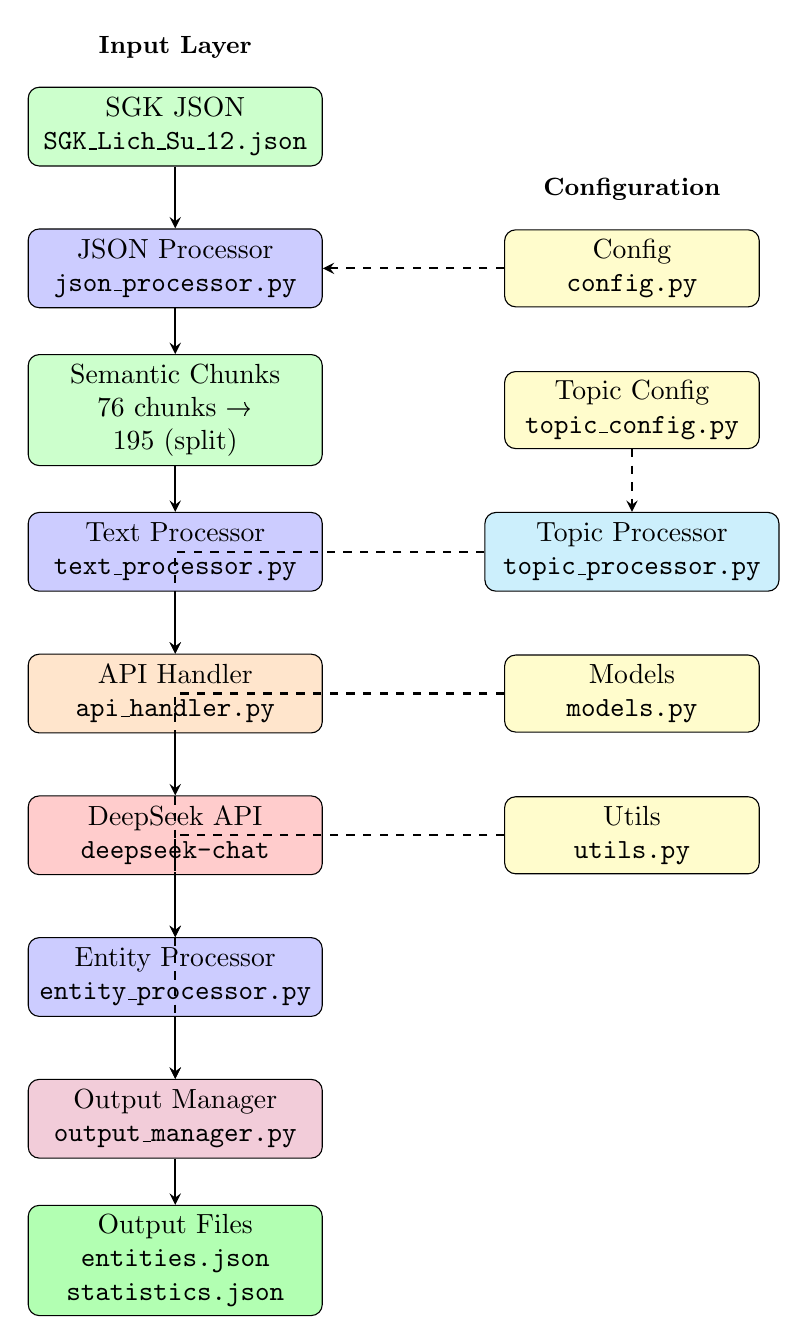
\begin{tikzpicture}[node distance=1.8cm, auto]
    % Styles
    \tikzstyle{datablock} = [rectangle, draw, fill=green!20, 
        text width=3.5cm, text centered, rounded corners, minimum height=1cm]
    \tikzstyle{component} = [rectangle, draw, fill=blue!20, 
        text width=3.5cm, text centered, rounded corners, minimum height=1cm]
    \tikzstyle{apiblock} = [rectangle, draw, fill=orange!20, 
        text width=3.5cm, text centered, rounded corners, minimum height=1cm]
    \tikzstyle{configblock} = [rectangle, draw, fill=yellow!20, 
        text width=3cm, text centered, rounded corners, minimum height=0.8cm]
    \tikzstyle{outputblock} = [rectangle, draw, fill=purple!20, 
        text width=3.5cm, text centered, rounded corners, minimum height=1cm]
    \tikzstyle{arrow} = [thick,->,>=stealth]
    \tikzstyle{dashedarrow} = [thick,->,>=stealth,dashed]
    
    % === LEFT COLUMN: Main Pipeline ===
    % Input Data
    \node [datablock] (input) {SGK JSON\\\texttt{SGK\_Lich\_Su\_12.json}};
    
    % JSON Processor
    \node [component, below of=input] (jsonproc) {JSON Processor\\\texttt{json\_processor.py}};
    
    % Semantic Chunks
    \node [datablock, below of=jsonproc] (chunks) {Semantic Chunks\\76 chunks → 195 (split)};
    
    % Text Processor
    \node [component, below of=chunks] (textproc) {Text Processor\\\texttt{text\_processor.py}};
    
    % API Handler
    \node [apiblock, below of=textproc] (apihandler) {API Handler\\\texttt{api\_handler.py}};
    
    % DeepSeek API (external)
    \node [apiblock, below of=apihandler, fill=red!20] (deepseek) {DeepSeek API\\\texttt{deepseek-chat}};
    
    % Entity Processor
    \node [component, below of=deepseek] (entityproc) {Entity Processor\\\texttt{entity\_processor.py}};
    
    % Output Manager
    \node [outputblock, below of=entityproc] (output) {Output Manager\\\texttt{output\_manager.py}};
    
    % Output Files
    \node [datablock, below of=output, fill=green!30] (outputfiles) {Output Files\\\texttt{entities.json}\\\texttt{statistics.json}};
    
    % === RIGHT COLUMN: Configuration & Support ===
    % Config
    \node [configblock, right of=jsonproc, xshift=4cm] (config) {Config\\\texttt{config.py}};
    
    % Topic Config Manager
    \node [configblock, below of=config] (topicconfig) {Topic Config\\\texttt{topic\_config.py}};
    
    % Topic Processor
    \node [component, below of=topicconfig, fill=cyan!20] (topicproc) {Topic Processor\\\texttt{topic\_processor.py}};
    
    % Models
    \node [configblock, below of=topicproc] (models) {Models\\\texttt{models.py}};
    
    % Utils
    \node [configblock, below of=models] (utils) {Utils\\\texttt{utils.py}};
    
    % === ARROWS: Main Flow ===
    \draw [arrow] (input) -- (jsonproc);
    \draw [arrow] (jsonproc) -- (chunks);
    \draw [arrow] (chunks) -- (textproc);
    \draw [arrow] (textproc) -- (apihandler);
    \draw [arrow] (apihandler) -- (deepseek);
    \draw [arrow] (deepseek) -- (entityproc);
    \draw [arrow] (entityproc) -- (output);
    \draw [arrow] (output) -- (outputfiles);
    
    % === ARROWS: Dependencies ===
    \draw [dashedarrow] (config) -- (jsonproc);
    \draw [dashedarrow] (topicconfig) -- (topicproc);
    \draw [dashedarrow] (topicproc) -| (apihandler);
    \draw [dashedarrow] (models) -| (entityproc);
    \draw [dashedarrow] (utils) -| (output);
    
    % === Labels ===
    \node [above of=input, yshift=-0.8cm, font=\small\bfseries] {Input Layer};
    \node [above of=config, yshift=-0.8cm, font=\small\bfseries] {Configuration};
    
\end{tikzpicture}
\caption{Kiến trúc tổng quan hệ thống Entity Extraction}
\label{fig:extract-architecture}
\end{figure}


\begin{figure}[H]
\centering
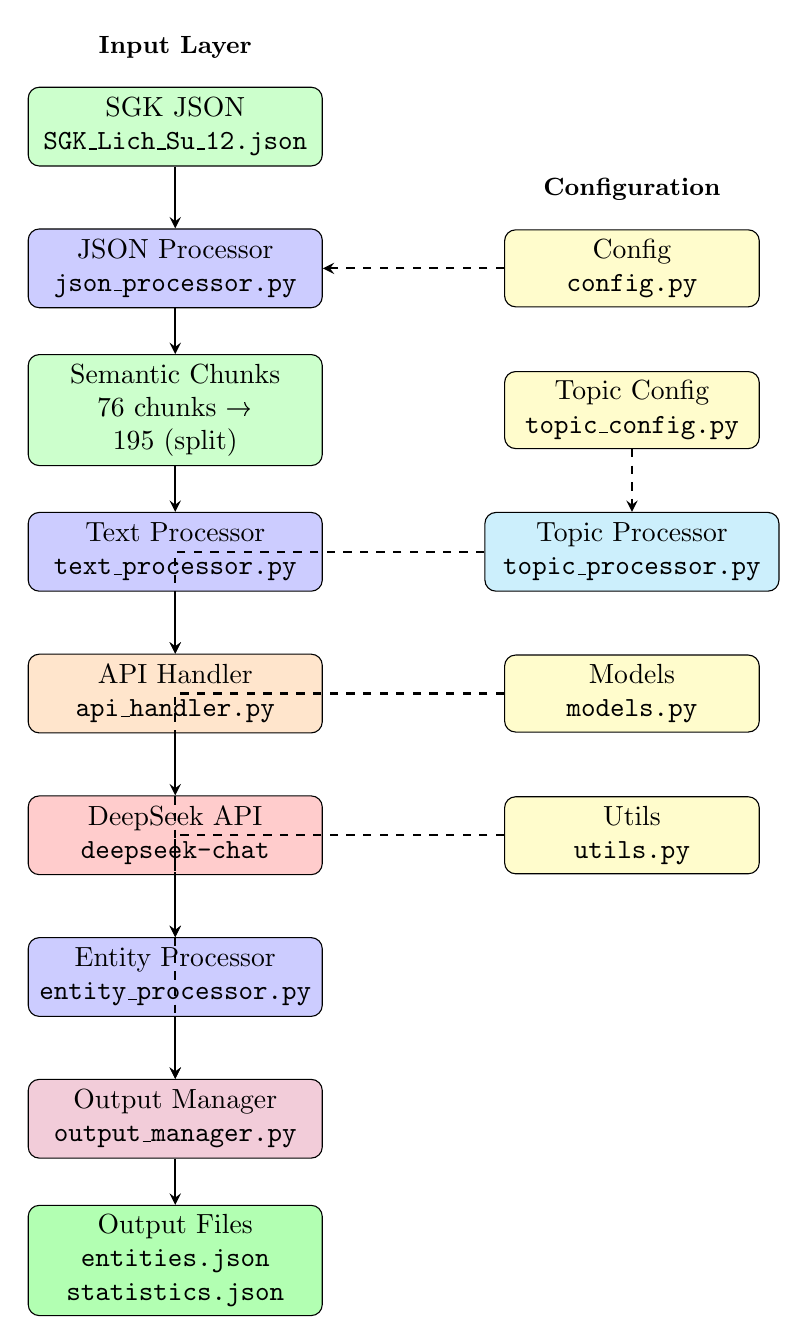
\begin{tikzpicture}[node distance=1.8cm, auto]
    % Styles
    \tikzstyle{datablock} = [rectangle, draw, fill=green!20, 
        text width=3.5cm, text centered, rounded corners, minimum height=1cm]
    \tikzstyle{component} = [rectangle, draw, fill=blue!20, 
        text width=3.5cm, text centered, rounded corners, minimum height=1cm]
    \tikzstyle{apiblock} = [rectangle, draw, fill=orange!20, 
        text width=3.5cm, text centered, rounded corners, minimum height=1cm]
    \tikzstyle{configblock} = [rectangle, draw, fill=yellow!20, 
        text width=3cm, text centered, rounded corners, minimum height=0.8cm]
    \tikzstyle{outputblock} = [rectangle, draw, fill=purple!20, 
        text width=3.5cm, text centered, rounded corners, minimum height=1cm]
    \tikzstyle{arrow} = [thick,->,>=stealth]
    \tikzstyle{dashedarrow} = [thick,->,>=stealth,dashed]
    
    % === LEFT COLUMN: Main Pipeline ===
    % Input Data
    \node [datablock] (input) {SGK JSON\\\texttt{SGK\_Lich\_Su\_12.json}};
    
    % JSON Processor
    \node [component, below of=input] (jsonproc) {JSON Processor\\\texttt{json\_processor.py}};
    
    % Semantic Chunks
    \node [datablock, below of=jsonproc] (chunks) {Semantic Chunks\\76 chunks → 195 (split)};
    
    % Text Processor
    \node [component, below of=chunks] (textproc) {Text Processor\\\texttt{text\_processor.py}};
    
    % API Handler
    \node [apiblock, below of=textproc] (apihandler) {API Handler\\\texttt{api\_handler.py}};
    
    % DeepSeek API (external)
    \node [apiblock, below of=apihandler, fill=red!20] (deepseek) {DeepSeek API\\\texttt{deepseek-chat}};
    
    % Entity Processor
    \node [component, below of=deepseek] (entityproc) {Entity Processor\\\texttt{entity\_processor.py}};
    
    % Output Manager
    \node [outputblock, below of=entityproc] (output) {Output Manager\\\texttt{output\_manager.py}};
    
    % Output Files
    \node [datablock, below of=output, fill=green!30] (outputfiles) {Output Files\\\texttt{entities.json}\\\texttt{statistics.json}};
    
    % === RIGHT COLUMN: Configuration & Support ===
    % Config
    \node [configblock, right of=jsonproc, xshift=4cm] (config) {Config\\\texttt{config.py}};
    
    % Topic Config Manager
    \node [configblock, below of=config] (topicconfig) {Topic Config\\\texttt{topic\_config.py}};
    
    % Topic Processor
    \node [component, below of=topicconfig, fill=cyan!20] (topicproc) {Topic Processor\\\texttt{topic\_processor.py}};
    
    % Models
    \node [configblock, below of=topicproc] (models) {Models\\\texttt{models.py}};
    
    % Utils
    \node [configblock, below of=models] (utils) {Utils\\\texttt{utils.py}};
    
    % === ARROWS: Main Flow ===
    \draw [arrow] (input) -- (jsonproc);
    \draw [arrow] (jsonproc) -- (chunks);
    \draw [arrow] (chunks) -- (textproc);
    \draw [arrow] (textproc) -- (apihandler);
    \draw [arrow] (apihandler) -- (deepseek);
    \draw [arrow] (deepseek) -- (entityproc);
    \draw [arrow] (entityproc) -- (output);
    \draw [arrow] (output) -- (outputfiles);
    
    % === ARROWS: Dependencies ===
    \draw [dashedarrow] (config) -- (jsonproc);
    \draw [dashedarrow] (topicconfig) -- (topicproc);
    \draw [dashedarrow] (topicproc) -| (apihandler);
    \draw [dashedarrow] (models) -| (entityproc);
    \draw [dashedarrow] (utils) -| (output);
    
    % === Labels ===
    \node [above of=input, yshift=-0.8cm, font=\small\bfseries] {Input Layer};
    \node [above of=config, yshift=-0.8cm, font=\small\bfseries] {Configuration};
    
\end{tikzpicture}
\caption{Kiến trúc tổng quan hệ thống Entity Extraction}
\label{fig:extract-architecture}
\end{figure}


\begin{figure}[H]
\centering
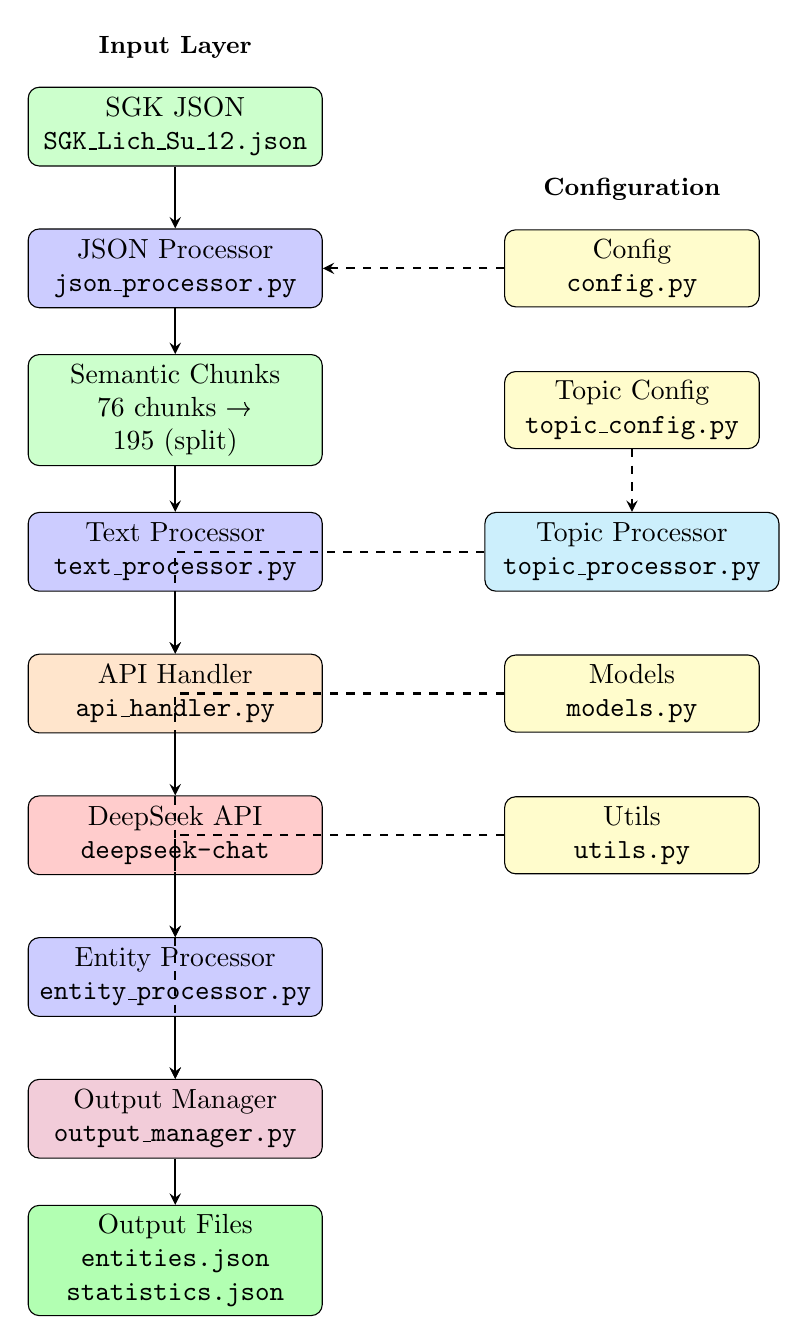
\begin{tikzpicture}[node distance=1.8cm, auto]
    % Styles
    \tikzstyle{datablock} = [rectangle, draw, fill=green!20, 
        text width=3.5cm, text centered, rounded corners, minimum height=1cm]
    \tikzstyle{component} = [rectangle, draw, fill=blue!20, 
        text width=3.5cm, text centered, rounded corners, minimum height=1cm]
    \tikzstyle{apiblock} = [rectangle, draw, fill=orange!20, 
        text width=3.5cm, text centered, rounded corners, minimum height=1cm]
    \tikzstyle{configblock} = [rectangle, draw, fill=yellow!20, 
        text width=3cm, text centered, rounded corners, minimum height=0.8cm]
    \tikzstyle{outputblock} = [rectangle, draw, fill=purple!20, 
        text width=3.5cm, text centered, rounded corners, minimum height=1cm]
    \tikzstyle{arrow} = [thick,->,>=stealth]
    \tikzstyle{dashedarrow} = [thick,->,>=stealth,dashed]
    
    % === LEFT COLUMN: Main Pipeline ===
    % Input Data
    \node [datablock] (input) {SGK JSON\\\texttt{SGK\_Lich\_Su\_12.json}};
    
    % JSON Processor
    \node [component, below of=input] (jsonproc) {JSON Processor\\\texttt{json\_processor.py}};
    
    % Semantic Chunks
    \node [datablock, below of=jsonproc] (chunks) {Semantic Chunks\\76 chunks → 195 (split)};
    
    % Text Processor
    \node [component, below of=chunks] (textproc) {Text Processor\\\texttt{text\_processor.py}};
    
    % API Handler
    \node [apiblock, below of=textproc] (apihandler) {API Handler\\\texttt{api\_handler.py}};
    
    % DeepSeek API (external)
    \node [apiblock, below of=apihandler, fill=red!20] (deepseek) {DeepSeek API\\\texttt{deepseek-chat}};
    
    % Entity Processor
    \node [component, below of=deepseek] (entityproc) {Entity Processor\\\texttt{entity\_processor.py}};
    
    % Output Manager
    \node [outputblock, below of=entityproc] (output) {Output Manager\\\texttt{output\_manager.py}};
    
    % Output Files
    \node [datablock, below of=output, fill=green!30] (outputfiles) {Output Files\\\texttt{entities.json}\\\texttt{statistics.json}};
    
    % === RIGHT COLUMN: Configuration & Support ===
    % Config
    \node [configblock, right of=jsonproc, xshift=4cm] (config) {Config\\\texttt{config.py}};
    
    % Topic Config Manager
    \node [configblock, below of=config] (topicconfig) {Topic Config\\\texttt{topic\_config.py}};
    
    % Topic Processor
    \node [component, below of=topicconfig, fill=cyan!20] (topicproc) {Topic Processor\\\texttt{topic\_processor.py}};
    
    % Models
    \node [configblock, below of=topicproc] (models) {Models\\\texttt{models.py}};
    
    % Utils
    \node [configblock, below of=models] (utils) {Utils\\\texttt{utils.py}};
    
    % === ARROWS: Main Flow ===
    \draw [arrow] (input) -- (jsonproc);
    \draw [arrow] (jsonproc) -- (chunks);
    \draw [arrow] (chunks) -- (textproc);
    \draw [arrow] (textproc) -- (apihandler);
    \draw [arrow] (apihandler) -- (deepseek);
    \draw [arrow] (deepseek) -- (entityproc);
    \draw [arrow] (entityproc) -- (output);
    \draw [arrow] (output) -- (outputfiles);
    
    % === ARROWS: Dependencies ===
    \draw [dashedarrow] (config) -- (jsonproc);
    \draw [dashedarrow] (topicconfig) -- (topicproc);
    \draw [dashedarrow] (topicproc) -| (apihandler);
    \draw [dashedarrow] (models) -| (entityproc);
    \draw [dashedarrow] (utils) -| (output);
    
    % === Labels ===
    \node [above of=input, yshift=-0.8cm, font=\small\bfseries] {Input Layer};
    \node [above of=config, yshift=-0.8cm, font=\small\bfseries] {Configuration};
    
\end{tikzpicture}
\caption{Kiến trúc tổng quan hệ thống Entity Extraction}
\label{fig:extract-architecture}
\end{figure}


\begin{figure}[H]
\centering
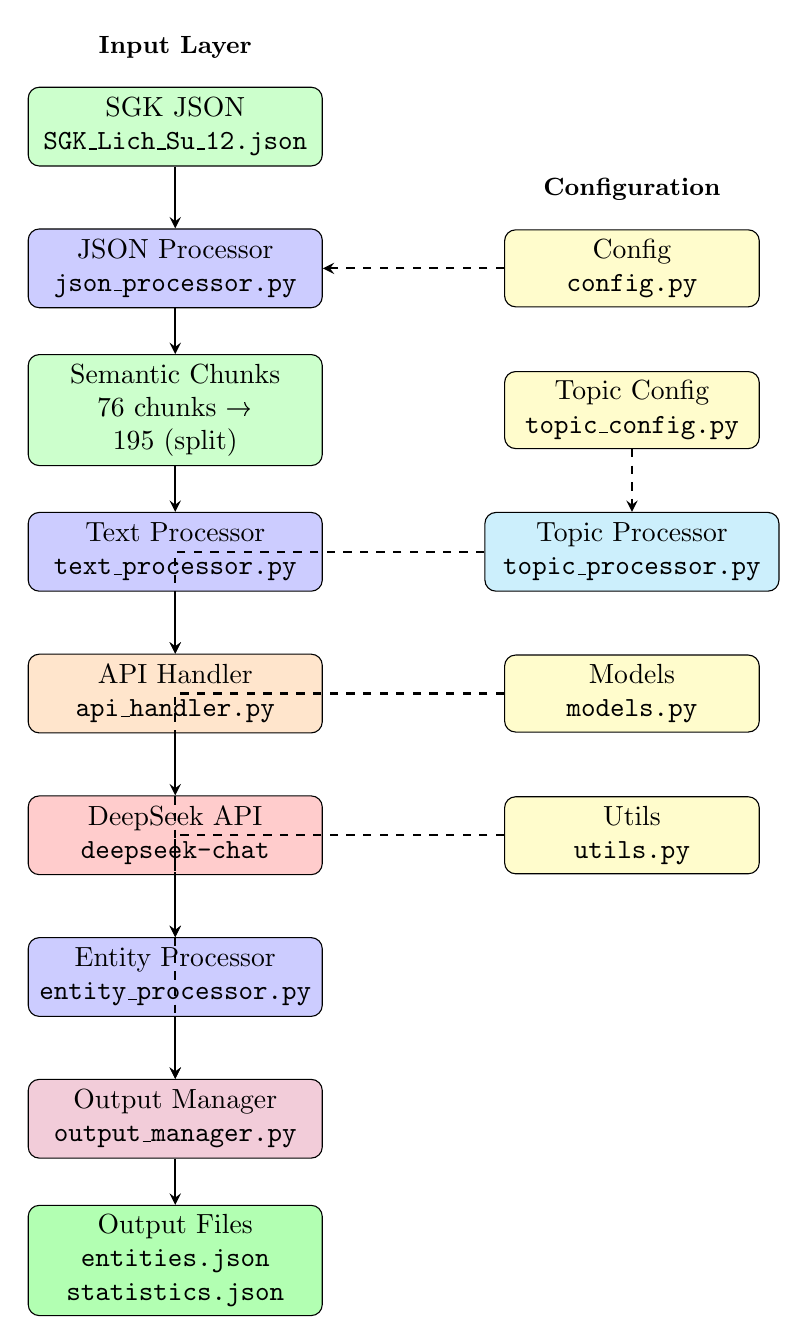
\begin{tikzpicture}[node distance=1.8cm, auto]
    % Styles
    \tikzstyle{datablock} = [rectangle, draw, fill=green!20, 
        text width=3.5cm, text centered, rounded corners, minimum height=1cm]
    \tikzstyle{component} = [rectangle, draw, fill=blue!20, 
        text width=3.5cm, text centered, rounded corners, minimum height=1cm]
    \tikzstyle{apiblock} = [rectangle, draw, fill=orange!20, 
        text width=3.5cm, text centered, rounded corners, minimum height=1cm]
    \tikzstyle{configblock} = [rectangle, draw, fill=yellow!20, 
        text width=3cm, text centered, rounded corners, minimum height=0.8cm]
    \tikzstyle{outputblock} = [rectangle, draw, fill=purple!20, 
        text width=3.5cm, text centered, rounded corners, minimum height=1cm]
    \tikzstyle{arrow} = [thick,->,>=stealth]
    \tikzstyle{dashedarrow} = [thick,->,>=stealth,dashed]
    
    % === LEFT COLUMN: Main Pipeline ===
    % Input Data
    \node [datablock] (input) {SGK JSON\\\texttt{SGK\_Lich\_Su\_12.json}};
    
    % JSON Processor
    \node [component, below of=input] (jsonproc) {JSON Processor\\\texttt{json\_processor.py}};
    
    % Semantic Chunks
    \node [datablock, below of=jsonproc] (chunks) {Semantic Chunks\\76 chunks → 195 (split)};
    
    % Text Processor
    \node [component, below of=chunks] (textproc) {Text Processor\\\texttt{text\_processor.py}};
    
    % API Handler
    \node [apiblock, below of=textproc] (apihandler) {API Handler\\\texttt{api\_handler.py}};
    
    % DeepSeek API (external)
    \node [apiblock, below of=apihandler, fill=red!20] (deepseek) {DeepSeek API\\\texttt{deepseek-chat}};
    
    % Entity Processor
    \node [component, below of=deepseek] (entityproc) {Entity Processor\\\texttt{entity\_processor.py}};
    
    % Output Manager
    \node [outputblock, below of=entityproc] (output) {Output Manager\\\texttt{output\_manager.py}};
    
    % Output Files
    \node [datablock, below of=output, fill=green!30] (outputfiles) {Output Files\\\texttt{entities.json}\\\texttt{statistics.json}};
    
    % === RIGHT COLUMN: Configuration & Support ===
    % Config
    \node [configblock, right of=jsonproc, xshift=4cm] (config) {Config\\\texttt{config.py}};
    
    % Topic Config Manager
    \node [configblock, below of=config] (topicconfig) {Topic Config\\\texttt{topic\_config.py}};
    
    % Topic Processor
    \node [component, below of=topicconfig, fill=cyan!20] (topicproc) {Topic Processor\\\texttt{topic\_processor.py}};
    
    % Models
    \node [configblock, below of=topicproc] (models) {Models\\\texttt{models.py}};
    
    % Utils
    \node [configblock, below of=models] (utils) {Utils\\\texttt{utils.py}};
    
    % === ARROWS: Main Flow ===
    \draw [arrow] (input) -- (jsonproc);
    \draw [arrow] (jsonproc) -- (chunks);
    \draw [arrow] (chunks) -- (textproc);
    \draw [arrow] (textproc) -- (apihandler);
    \draw [arrow] (apihandler) -- (deepseek);
    \draw [arrow] (deepseek) -- (entityproc);
    \draw [arrow] (entityproc) -- (output);
    \draw [arrow] (output) -- (outputfiles);
    
    % === ARROWS: Dependencies ===
    \draw [dashedarrow] (config) -- (jsonproc);
    \draw [dashedarrow] (topicconfig) -- (topicproc);
    \draw [dashedarrow] (topicproc) -| (apihandler);
    \draw [dashedarrow] (models) -| (entityproc);
    \draw [dashedarrow] (utils) -| (output);
    
    % === Labels ===
    \node [above of=input, yshift=-0.8cm, font=\small\bfseries] {Input Layer};
    \node [above of=config, yshift=-0.8cm, font=\small\bfseries] {Configuration};
    
\end{tikzpicture}
\caption{Kiến trúc tổng quan hệ thống Entity Extraction}
\label{fig:extract-architecture}
\end{figure}
